\chapter{Results and discussions} \label{chapter6}

Following subsections shall discuss in detail, the various conclusions that were inferred by the developers/designers from the present investigation, a brief overview of the methodologies learned, deviations from ideality (if any), safety precautions which were followed and a creator’s road map for implementation of a similar project and other moderately or less important details.


\section{Basic inferences}

The following list has been divided into two main sub-lists, namely a set of direct inferences (those inferences which are easily derived by following the normal development road map) and a set of indirect inferences (those inferences which need a deeper understanding of the application requirements of the project).

\subsection{Direct inferences}

\subsubsection*{D1 – Large sized assemblies must be supported by suitable base material} \label{first_inf}

It is obvious from section \ref{bmaterial} that the piece of polished wood is optimal for the base material design. The two main reasons to support this claim are

\begin{itemize}
 \item Wood as a material, when used with considerable and uniform dimensions forms a good integrating platform on which other \textit{heavy machinery} can be mounted. Heavy machinery here refers to any object of considerable weight and dimensions which easily couples with the wooden material either by means of screw fastening mechanisms or directly integrated into slots made into the material. The bottom line is that both types of component material whether similar or dissimilar to wood, wood forms a natural integrating platform for all.
 \item Wood is light (has lesser weight in comparison with the sum of weights of other discrete components), sturdy, easy to clean as well as rests easily on a flat surface.
\end{itemize}

Hence, the choice of the base material.

\subsubsection*{D2 – Usage of buffered dimensions instead of going for exact measurements}

This point has been reiterated through the entire report in various sections of importance. The reasons pertaining to consideration of buffered dimensions is that it always leaves out a tolerance band for error, i.e. even if some form of error creeps in due to improper or faulty machining work of a wide variety of instruments, they can be rectified easily. Although any form of error may lead to material wastage it is still way better than a faulty piece of material which is fundamentally useless and needs a replacement altogether. The downside is that the sum of all buffered dimensions would create a moderate to a large increase in overall dimensions of the entire physical structure/assembly thereby also hampering its overall portability.

\subsubsection*{D3 – Choice of proper adhesive material}

As stated in section \ref{screws} a suitable material should be chosen for such purposes. Various types of fast-drying glue may seem to be an intuitively easy option however, they don’t stand the test of time and are not viable in the long run. Therefore, throughout the entire assembly screws have been used for fixing and coupling together components of similar and dissimilar materials.

\subsubsection*{D1 – Optimum power supply}

As stated multiple times in section \ref{psupply} a single power supply should be sufficient for the entire project. However, designing a dedicated PCB for the purpose would have been simply tedious and time-consuming and hence was omitted for the current iteration of the project. But at the same time this increased density of power lines and cables. Additionally, it should be noted that power supply units are in general bulky and heavy for e.g. adapters, single/dual regulated supplies etc. So it pays off to design a single dedicated circuit for all such powering purposes.


\subsection{Indirect inferences}

\subsubsection*{ID1 – Consideration of weight capacity of stepper motors}

This point has not been stated anywhere else in the report, however, a little insight into what all would be coupled with a stepper motor shaft tells us that it will be bearing a considerable amount of heavy loads.The stepper motor assigned for the X-axis segment must be able to rotate a coupled rod, resting on which is the entire Y-axis segment (a part of whose weight is resting on this threaded rod and another smooth support rod). Invariably and indirectly the stepper motor for the X-axis is supporting the weight of both the rods as well as the weight of the complete Y-axis segment. So a large capacity stepper motor needs to be considered.The stepper motor for the Y-axis segment is relatively less constrained in terms of weight capacity and any suitable capacity motor which can rotate a threaded rod will do.

\subsubsection*{ID2 – Stability of the entire structure}

A little thought has been given to this part however while the CNC drill engraves tracks on the PCB, it should be noted that tremendous amounts of vibrations are produced in the system. A sturdy base material does help as stated in \ref{first_inf} D1 however, additional counterbalance weights at strategic positions is suggested for enhanced stability.

\subsubsection*{ID3 – Engraving and drilling bits}

The review from section \ref{res_and_acc} should be taken into account while discussing engraving and drilling bits. There are two points to be kept in mind while choosing these bits for a CNC machine: the dimensions and the material. The ideal material is Tungsten Carbide although it is expensive. Drills for glass cutting and engraving may not be always suitable for PCB engraving purposes. For understanding what dimensions would be appropriate for the various engraving bits an iterative approach could be taken up. With the \textit{available bits}, the smallest and largest possible wire thicknesses should be engraved. If the output quality is within the acceptable error limits set by the designers then the available set of bits is sufficient for the machine. If it is not, choose finer and harder bits for the same purpose and repeat the above process. Continue until the desired quality of output is obtained. Choose these engraving and drilling bits for your CNC machine.

\section{Safety precautions undertaken}

Throughout the potentially hazardous phase of the machining work, the operators of various machining tools, as well as the designers of the project, took multiple safety precautions. Following is a recommended set of safety precautions that must be followed whenever similar kind of projects is undertaken:

\begin{enumerate}
 \item Only experts and professional operators who are familiar with the machine should handle it under all circumstances.
 \item Keep a safe distance from rotating lathes, metal drills while they are in operation at least by 1.5 to 3 ft.
 \item While large-sized machinery is in operation, maintain a safe distance from its HV power supply.
 \item For rotating spindles, drill bits, etc. always make it a habit to spray lubricant on which the job is being done.
 \item Vices, holders, metallic jaws and other such similar equipment always pose a pinching hazard, handle them carefully.
 \item As a general rule, look up to the safety of yourself and others and be fully aware of your surroundings.
\end{enumerate}

\section{Standard testing procedures}

Testing for any project is always divided into two major parts: each of the small components (either software or hardware) is tested at an individual level which is termed as unit testing. And after the given project has been completed successfully, its entire performance is judged or inspected end-to-end which is termed as full testing or integrated testing. The procedure for unit testing of various components (and the results obtained from them) are mentioned below. The reasons for incomplete full testing have also been mentioned in the following section.

\subsection{Unit Testing}

\subsubsection*{Testing of motors}

It should be noted that motors \textbf{should not} be tested until and unless the calibration of the motor drivers as mentioned in \ref{motor_calib} is fully complete. After the calibration has been completed, both the stepper motors should be interfaced as mentioned in \ref{winterface}. Now it should be noted that the rotation of the motor shafts needs to be tested for both \textit{coarse} and \textit{fine} movements of the drill head on the copper clad. A typical coarse movement could be drawing the outline cut (section \ref{outline_cut}) for a PCB while a fine movement could be drawing any trace width of minute dimensions. Rotation of the motor is very clearly visible for the former, however, for fine movements, the rotation may not be visible. To visualise the same, a paper or a cardboard sheet with the name of the axis written on it must be attached to the motor shafts. A clockwise arrow should be drawn as well. This will ensure that even minor rotations (in either direction) would be visible as the cardboard piece shall rotate with the shaft. Following is an image representing the same. \par

\begin{figure}[h]
 \centering
 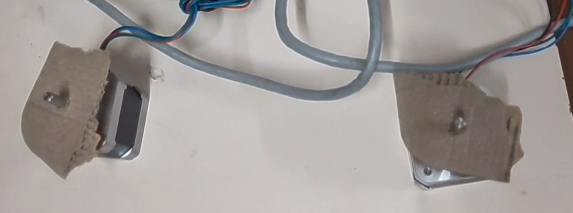
\includegraphics[scale = 0.75]{Chapter_6/motor_label.png}
 \caption{An illustration of how rotation of stepper motors is verified visually using cardboard labels during testing}
 \label{fig:motorlabel}
\end{figure}

A similar testing routine was developed for the stepper motors of this CNC machine. It was tested using the CAM processor software’s \textit{jog controller} feature. Using the jog controller gave the designers an ability to provide fine movement to both the stepper motors (in both the directions) as well as coarse movements by long-pressing any of the controller buttons on the software.The working of the motors was successfully tested and their performance was within their nominal design limits.

\subsubsection*{Testing of G code generation software}

Testing of software is relatively easy as compared to working hardware. For testing the G-code generation software (described in section \ref{gcodegen}), two PCB Gerber files were generated from schematic design software and were fed into the web application. The first Gerber file corresponded to an RC circuit which is relatively simple to design while the second one belonged to a relatively complex PCB design i.e. an intruder alarm circuit (the one illustrated in figure \ref{fig:ckt_brd}). In both cases, the settings regarding the copper-clad thickness, tool dimensions and extra features such as outline-cut were kept exactly the same. \par

The G-code generated for both the PCBs were judged in terms of size and quality. The testing of the software after the inspection was deemed to be successful and very much within its design limits.

\subsubsection*{Testing of CAM processor software along with unit components}

The CAM processor software is quite vast so the testing of only the features relevant to this project has been detailed here. The main features of this software are the code editor, visualiser, jog controller and a display showing the real-time coordinates of the tooltip in appropriate units. Following is a brief description of how they were tested. \par

To begin with, the G-code file corresponding to the RC circuit from the previous step was uploaded in the software. All the functionality relating to connecting the CNC setup to the PC is verified. This may include (depending on the software) a COM port indicator, baud rate indicator, an icon denoting successful connection etc. After verifying these settings the code editor that is present onboard can be tested. \par

To test the editor, deleting, adding, commenting and editing a few lines is recommended. If the editor saves them in realtime then the testing is deemed to be successful. Following that the jog controller can be tested. One by one each of the directional buttons (+/-) corresponding to each of the three axes are tested. If the relevant motors are rotating in the required directions then it can be concluded that the jog controller is working properly. The same was done for this CNC setup as well. \par

After all the pre-operation steps are completed then only is it possible to test the live visualiser and the indicators showing the controller states. After clicking on the run button, the G-code program starts running. If all goes well, depending on the complexity of the program and the PCB, the entire program may run in excess of five minutes. The real-time machine status is indicated on the \textbf{DRO controller} where the coordinates of the tooltip would be displayed in double-digit precision. At the same time, live visualiser can be tested. The entire tool path is visible in yellow (which is precomputed once the G-code is loaded) and only the tooltip is shown. If with the rotation of the motors, appropriate movement of the tooltip is visible on the visualiser then it is highly probable that the CNC set up along with the software is working absolutely fine. However, to completely ensure that the CAM processor software is working properly, integrated or full testing would be required.All the aforementioned steps were followed to ensure that the CAM processor software was working properly. The CAM processor software testing was deemed to be successful.


\subsection{Integrated or full testing}

As stated at the beginning of this section, testing of components used to make up a system is a multistage and iterative process as opposed to a single-step process. While testing the motors described in section \ref{step_motors} it was realised that for coarse movements, the capacity of the stepper motor for the X-axis was insufficient to rotate a heavy threaded rod. Added to this was the fact that an entire identical axis assembly would have been loaded on this axis. Clearly the NEMA 17 stepper motor variants were incapable of this job. An ideal upgrade could have been the NEMA 23 variants. However, due to time constraints, the same could not be procured in the available period and \textbf{hence the project, as well as its integrated or full testing, remains incomplete}.

\section{Test case selection}

For any given project, testing is invaluable. However, the procedures to be followed for the same are equally important and should be documented well. The reason being that any system has various levels of limitations. It is important to provide test inputs in a way that is within the nominal limits of operation of a machine. In a similar fashion, it is also expected that the output would be within the design limits for the precision and accuracy of the machine. For our CNC machine, we have highlighted some important points to follow and remember while testing our project. These points would also be beneficial to someone who wants to design a dedicated testing rig for a similar such system. \cite{online_book}

\begin{enumerate}
 \item The CNC machine can only handle single-layer PCBs - As of now (stated multiple times in this report) this CNC machine is capable of milling only single-sided or single-layer PCBs. Therefore, it should not be tested against G-code obtained from multilayer PCBs. To genuinely emulate milling of multilayered PCBs, the tester can generate G-code of individual layers (a feature of all common schematic design software) and test the same on our machine. Following is how a  and  test case looks like.

       \begin{figure}[h]

        \begin{subfigure}{0.5\textwidth}
         \hspace{8mm}
         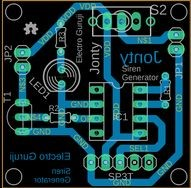
\includegraphics[width=0.8\linewidth, height=6cm]{Chapter_6/eagle_single.jpg}
         \caption{Single layered PCB}
         \label{fig:slpcb}
        \end{subfigure}
        \begin{subfigure}{0.5\textwidth}
         \hspace{8mm}
         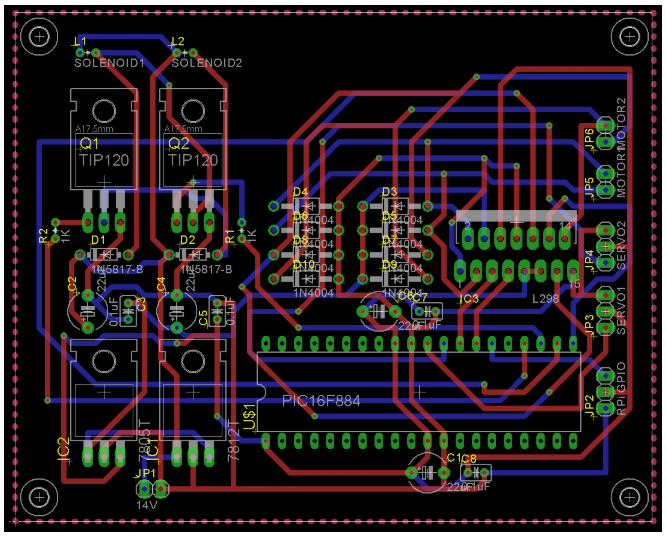
\includegraphics[width=0.8\linewidth, height=6cm]{Chapter_6/eagle_double.png}
         \caption{Double layered PCB}
         \label{fig:dlpcb}
        \end{subfigure}

        \caption{The two illustrations above represent what could be a good and a bad test case respectively for the first rule}
        \label{fig:sl_dl_pcb}
       \end{figure}

 \item The CNC machine doesn’t automatically rectify issues in PCB design - The rules and guidelines for creating a really nice industry-grade PCB are large in number. Every PCB given as an input may not obey the said specifications. There could be faults in corners, tracks, track spaces etc.. These problems (and rectification of the same) is the sole responsibility of the user/tester and it should be noted that the software associated with the CNC machine is not capable of understanding the same. If an inappropriately designed PCB (satisfying the previous rule) is given as an input, an equivalent output would be generated within the design limits of the CNC machine. The software doesn’t include any image processing routines and hence no errors would be rectified automatically. Following is an example of what could be a \textit{good} and \textit{bad} test case in this scenario.

       \begin{figure}[h]

        \begin{subfigure}{0.5\textwidth}
         \hspace{8mm}
         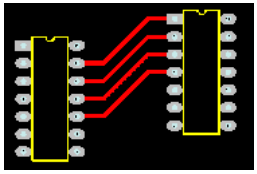
\includegraphics[width=0.8\linewidth, height=6cm]{Chapter_6/eagle_good_rout.png}
         \caption{Components with good routing}
         \label{fig:grout}
        \end{subfigure}
        \begin{subfigure}{0.5\textwidth}
         \hspace{8mm}
         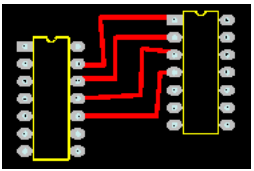
\includegraphics[width=0.8\linewidth, height=6cm]{Chapter_6/eagle_bad_rout.png}
         \caption{Components with bad routing}
         \label{fig:brout}
        \end{subfigure}

        \caption{The two illustrations above represent what could be a good and a bad test case respectively for the second rule}
        \label{fig:gbrout}
       \end{figure}

 \item G-code containing machine codes - While testing this CNC machine it should be noted that it doesn’t include any advanced machine control functions such as \textit{spindle control}, \textit{coolant ON/OFF}, \textit{tool change} etc. although the CNC shield has ports for the same. However, the generated G-code may very often have machine codes indicating one or multiple of the above operations. It is the responsibility of the tester to ensure that such lines of code are commented OR are removed from the program in their entirety. Additionally, some codes belong to different G-code versions and are not compatible with all machines. Such G-codes \textbf{should be} replaced with suitable alternatives.

 \item Placement of the machine on a straight and flat surface - For all testing regimes it should always be ensured that the CNC machine is placed on a straight and flat surface which is (preferably) heavy and stable. Although the machine has a baseboard of large dimensions made using wood, the copper-clad itself could have minor and major aberrations or non-uniformities on its surface. Although procedures like auto levelling and others have been mentioned in the literature review, those features could not be implemented due to time constraints. Hence, ensuring a proper flat surface during testing or normal operation is the sole responsibility of the user. Following are images showing what a \textit{good} and \textit{bad} test case would look like.

       \begin{figure}[h]

        \begin{subfigure}{0.5\textwidth}
         \hspace{8mm}
         
\includegraphics[width=0.8\linewidth, height=6cm]{Chapter_6/proper_clad.png}
         \caption{Clean PCB copper cladding which is straight and flat}
         \label{fig:pclad}
        \end{subfigure}
        \begin{subfigure}{0.5\textwidth}
         \hspace{8mm}
         
\includegraphics[width=0.8\linewidth, height=6cm]{Chapter_6/improper_clad.png}
         \caption{An unclean PCB copper cladding which may have micro bends and abrasions on its surface}
         \label{fig:iclad}
        \end{subfigure}

        \caption{The two illustrations above represent what could be a good and a bad test case respectively for the fourth rule}
        \label{fig:piclad}
       \end{figure}

\end{enumerate}

The above guidelines, if followed properly are sufficient to carry out proper testing for the CNC machine.

\section{Scope for future work}

Although the project was completed it does leave out on many critical points wherein it could have been improvised. Following are some points which can be looked upon by any designer or developer who would like to further develop the project. These key points are only a few of those areas where primary development should be focused on and doesn’t necessarily include everything where improvisation could be carried out (that is left as an exercise to developers).

\begin{enumerate}
 \item Develop a proper PSU for the entire system.
 \item Develop a single PCB containing the entire circuitry to control the system.
 \item Use a more powerful and dedicated drilling motor for the actual engraving purpose.
 \item Develop a single integrated software platform for the entire engraving process which facilitates every step from G-code generation to the final PCB output.
 \item Optimise or develop G-code generation routines which can handle multiple PCBs at the same time without any manual intervention till their net dimensions are within 15 cm x 15 cm.
 \item Improvise necessary hardware and/or software to handle multi-layered PCBs.
 \item Improvise necessary hardware and/or software to carry out the special procedures listed in section \ref{spec_proc} automatically.
 \item Develop a proper enclosure for the entire CNC machine if possible with cooling and vacuuming systems.
\end{enumerate}
